\DiaryEntry{Prefix Codes - Intuition}{2021-04-26}{Coding}

\subsection{Code Construction}

We consider prefix codes and play around with some examples. We start with a code for $3$ symbols as in the folloing Figure, upper part.

This is a prefix code as all codewords are at the leaves of the tree. We continue using the convention from the previous entry that a left turn corresponds to a $0$ and a right turn corresponds to a $1$. So the codeword for symbol $B$ is $01$ (left-right).

\begin{figure}[H]
    \centering
    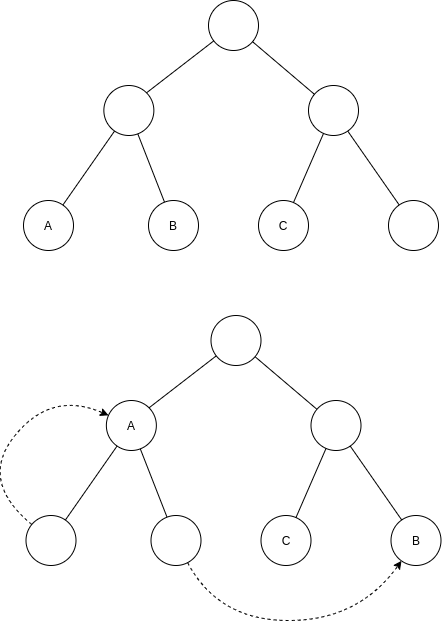
\includegraphics[scale=0.4]{images/2021-04-26-scenario_1.png}
\end{figure}

Assume that symbol $A$ has a higher probability and we decide to assign it a shorter codeword. We therefore move it up in the tree (see lower part of the Figure) so that the codeword becomes $0$. Since we want a prefix code, we have to move symbol $B$ from its current position so that it does not stay below $A$. We therefore move $B$ to a currently unused tree node (codeword $11$).

As a whole, the average codeword length has decreased: Symbols $B, C$ have codewords of the same length assigned and symbol $A$ has a codeword of length $1$ assigned.

This example was easy, as we had enough room in the tree to accomodate symbol $B$. The next example is a bit more involved.

The initial assignment is shown in the upper part of the following Figure. We again decide to assign symbol $A$ the shorter codeword $0$ (instead of $000$). Now we have to move symbols $B, C, D$ to another place in the tree. We move symbol $B$ from $001$ to $110$. Symbols $C$ and $D$ are a bit more complex as we have only one more vacancy with codelength $3$ in the tree. We therefore need to introduce a further level in the tree and move symbol $C$ to $1110$ and symbol $D$ to $1111$.

\begin{figure}[H]
    \centering
    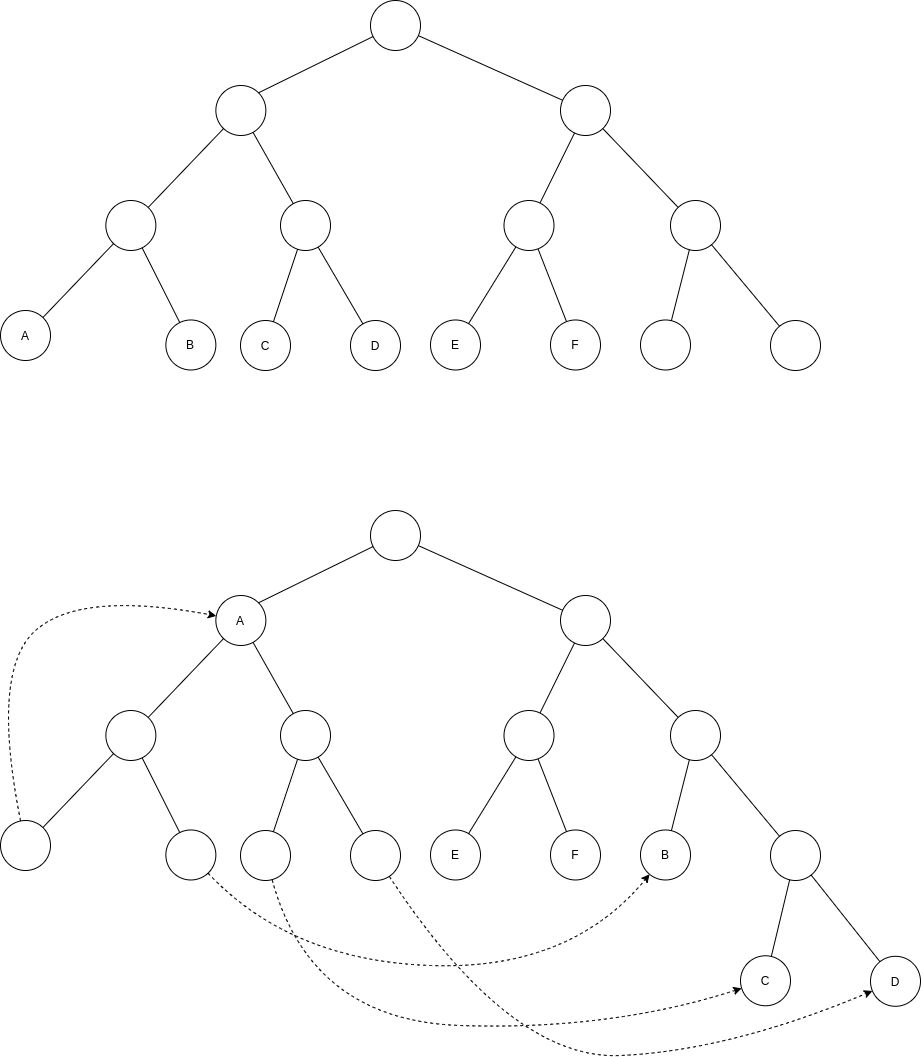
\includegraphics[scale=0.4]{images/2021-04-26-scenario_2.png}
\end{figure}

In this case, we cannot make a statement about the average codeword length: We have shortened the codeword for symbol $A$, however, the codeword length for symbols $C, D$ has increased. Without knowing the symbol probabilities, we cannot say which effect is stronger.

In addition, maybe it would have been better to move another symbol to where we have moved symbols $C$ and $D$ and / or restructure the tree more fundamentally. The Huffman code construction starts bottom-up (i.e. with the symbols having lowest probability first) and does not rework an already existing tree. Therefore a Huffman code may yield a different result in this case.


\subsection{Kraft-McMillian Inequality}

We have already discussed the inequality; here we give the proofs. The first part is not so interesting: We are given a code $\Cc$ with $N$ codewords of length $l_1, l_2, \ldots, l_N$. If $\Cc$ is uniquely decodable, then

\bee
    K(\Cc) = \sum_i 2^{-l_i} \leq 1
\eee

The proof works by looking at the $n$-th power of $K(\Cc)$. If $K(\Cc) > 1$, then $K(\Cc)^n$ would grow exponentially with $n$. If it does not grow exponentially with $n$, then this is proof that $K(\Cc) = \sum_i 2^{-l_i} \leq 1$.

Let $n$ be an arbitrary integer. Then we have

\bee
\left[ \sum_i 2^{-l_i} \right]^n = \left( \sum_{i_1} 2^{-l_{i_1}} \right) \cdots \left( \sum_{i_n} 2^{-l_{i_n}} \right) = \sum_{i_1} \cdots \sum_{i_n} 2^{-(l_{i_1} + \cdots + l_{i_n})}
\eee

The exponent $l_{i_1} + \cdots + l_{i_n}$ is simply the length of $n$ codewords from the code $\Cc$. The smallest value that this exponent can take is greater than or equal to $n$, which would be the case if all codewords were $1$ bit long. If

\bee
l = \max\{ l_{i_1}, \ldots, l_{i_n} \}
\eee

then the largest value the exponent can take is less than or equal to $nl$. Therefore, we can write above summation as

\bee
K(\Cc)^n = \sum_{k=n}^{nl} A_k 2^{-k}
\eee

where $A_k$ is the number of combinations of $n$ codewords that have a combined length of $k$. Let’s take a look at the size of this coefficient. The number of possible distinct binary sequences of length $k$ is $2^k$. If this code is uniquely decodable, then each sequence can represent one and only one sequence of codewords. Therefore, the number of possible combinations of codewords whose combined length is $k$ cannot be greater than $2^k$. In other words, we have

\bee
A_k \leq 2^k
\eee

Inserting this into the epxression for $K(\Cc)^n$, we obtain

\bee
K(\Cc)^n = \sum_{k=n}^{nl} A_k 2^{-k} \leq \sum_{k=n}^{nl} 2^k 2^{-k} = nl - n +1
\eee

But if $K(\Cc)$ is greater than one, it will grow exponentially with $n$, while $n(l − 1) + 1$ can only grow linearly. So if $K(\Cc)$ is greater than one, we can always find an $n$ large enough so that above inequality is violated. Therefore, for a uniquely decodable code $\Cc$, $K(\Cc)$ is less than or equal to one. \qed


The second part of the inequality is that if we have a set of codeword lengths that satisfy the inequality, we can always find a prefix code with those codeword lengths.


Given a set of integers $l_1, l_2, \ldots, l_N$ fulfilling

\bee
    K(\Cc) = \sum_i 2^{-l_i} \leq 1
\eee

then we can always find a prefix code with codeword lengths $l_1, l_2, \ldots, l_N$.

For the proof we will develop a procedure for constructing a prefix code with code-word lengths $l_1 , l_2, \ldots, l_N$ that satisfy the given inequality. We will assume, without loss of generality, that $l_1 \leq l_2 \leq \cdots \leq l_N$. 


The following Figure shows a binary tree of depth $4$. 

\begin{figure}[H]
    \centering
    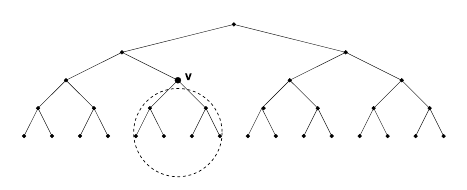
\includegraphics[scale=0.4]{images/2021-04-26-tree.png}
\end{figure}

The number of leaf nodes on this tree is $2^4 = 8$. In fact the number of leaf nodes in a full binary tree of depth $m$ is $2^m$ . We will construct our code by assigning vertices at depth $l_i$ as codewords. In order for this code to be a prefix code when we assign a code to a vertex within the tree we cannot assign a codeword to any leaves belonging to the sub-tree rooted at that node. In effect, we have to prune the subtree rooted at that vertex. For example if we assign a codeword to the vertex $v$ indicated in the figure we have to remove the subtree shown in the dashed circle. In the figure the vertex $v$ is at depth two. The removal of the corresponding subtree results in the removal of four leaf nodes. In general we can see that in a full binary tree of depth $m$, a vertex at depth $k$ is the root of a subtree with $2^{m−k}$ leaves.

Given the set of lengths $l_1, l_2, \ldots, l_N$, we define $l = \max\{ l_1, l_2, \ldots ,l_N \}$ and construct a binary tree of depth $l$. This tree has $2^l$ leaves, and hence the possibility of having $2^l$ codewords of length $l$. Let’s assign a codeword to a vertex $v_1$ at depth $l_1$. The path from the root node of the tree to this vertex will be a binary code of length $l_1$. As we mentioned earlier in order for this codeword to be part of a prefix code we need to prune the subtree rooted at node $v_1$. This will result in a loss of $2^{l−l_1}$ leaf nodes from the full binary tree of depth $l$. Assign the next codeword to a vertex $v_2$ at a depth of $l_2$ and prune the subtree rooted at $v_2$. Continuing in this fashion we will obtain a prefix code with lengths $l_1, l_2, \ldots, l_N$ as long as we don’t use up more than $2^l$ leaf nodes. As a codeword of length $l_i$ results in the loss of $2^{l−l_i}$ leaf nodes from the full tree, the number of leaf nodes needed to build a code with codeword lengths $l_11, l_2, \ldots, l_N$ is given by $\sum_i 2^{l−l_i}$, but

\bee
\sum_i 2^{l−l_i} = 2^l \sum_i 2^{−l_i} \leq 2^l
\eee

where the last inequality is because of our assumption that the lengths satisfy the Kraft–McMillan inequality. Thus, given a set of codeword lengths satisfying the Kraft–McMillan inequality we can always construct a prefix code with codewords having those lengths. \qed

%%% Local Variables:
%%% mode: latex
%%% TeX-master: "journal"
%%% End:
